\documentclass[journal]{IEEEtran} % use the `journal` option for ITherm conference style
\IEEEoverridecommandlockouts
% The preceding line is only needed to identify funding in the first footnote. If that is unneeded, please comment it out.
\usepackage{cite}
\usepackage{amsmath,amssymb,amsfonts}
\usepackage{algorithmic}
\usepackage{graphicx}
\usepackage{CJKutf8}
\usepackage{textcomp}
\usepackage{xcolor}
\def\BibTeX{{\rm B\kern-.05em{\sc i\kern-.025em b}\kern-.08em
    T\kern-.1667em\lower.7ex\hbox{E}\kern-.125emX}}
\begin{document}

\begin{CJK*}{UTF8}{gbsn}

\title{Hiding Sensitive Information in Desensitized Voice Sequences}

\author{%%%% author names
    \IEEEauthorblockN{1\textsuperscript{st} Given Name Surname}% first author
    , \IEEEauthorblockN{2\textsuperscript{nd} Given Name Surname}% delete this line if not needed
    , \IEEEauthorblockN{3\textsuperscript{rd} Given Name Surname}% delete this line if not needed
    % duplicate the line above as many times as needed to list all authors
    \\%%%% author affiliations
    \IEEEauthorblockA{\textit{dept. name of organization (of Aff.), City, Country}}\\% first affiliation
    \IEEEauthorblockA{\textit{dept. name of organization (of Aff.), City, Country if needed}}\\% delete this line if not needed
    % duplicate the line above as many times as needed to list all affiliations
    %%%% corresponding author contact details
    \IEEEauthorblockA{email address or ORCID of corresponding author(s)}
}

\maketitle

\textbf{DRAFT VERSION III}

\begin{abstract}
Voice data is broadly acquired and utilized by consumer services. In order to process such data, most of the raw records are sent to web servers, possibly with dedicated acceleration hardware. However, in this way malicious service providers can identify the users because the raw voice sequences contain rich voiceprint information, which is adequate for deduction of a large amount of private information. In order to mitigate such problem, desensitization methods are employed as secure intermediaries between user and the cloud services. However, if these methods are provided by a third party as a black box, it may not proved to be safe enough. In this paper, we demonstrate and experiment the possibility of hiding information sufficient to extract original voice from in seemingly desensitized voices that may be used for various online services, utilizing StarGAN-based voice transformation and voice-optimized audio stenography technologies.
\end{abstract}

\begin{IEEEkeywords}
    privacy, voice, desensitization, stenography
\end{IEEEkeywords}

\section{Introduction}
Voice has been one of the most important means of human-machine interaction. With the rapid development of deep-learning means, there are now a large number of voice recognition and manipulation technologies.

Particularly, voiceprint analysis enabled effective association of human identity to their voices, thus led to the possibility of voice-only authentication. This type of authentication allows users to omit traditional password-based security factor, thereby avoided associated concerns like weak passwords or the lack of regular modification. Also, the need for users to recall a robust and secure sequence of password is thus eliminated.

Some voice-based services use voiceprint to prevent unwanted activations,such as Siri from Apple Inc. and Xiao Ai from Xiaomi Inc.\cite{a19, a20}. Also, there are many voice enabled IMEs for various kinds of devices, such as iFly Input Method from iFlyTek and GBoard from Google, Inc.\cite{a21, a22}. Also deep learning-based speech synthesis have made great progress. With state of the art techniques, it's not easy to distinguish the speech sequences produced by the generation-oriented services.\cite{a12}.

However, such advancement in other hand reminds people of the feature-rich nature of raw voice recordings and the vulnerabilities born from them\cite{a6, a7}. These sequences contains enormous amount of sensitive personal information, and if they are processed by a untrusted party, the likelihood of data exposure and leaking is high.

The decisive solution to this problem would involve performing the entire process locally on user's device. However, such services would not likely to lightweight enough to be able to operated in this way. It's unavoidable that certain parts of workflow of such services will have to be done remotely, and potentially cause security issues. For example, Xiaomi claims that Xiao Ai can "do most of the training and evaluation locally" \cite{a20}.

\begin{figure}[htbp]
    \centerline{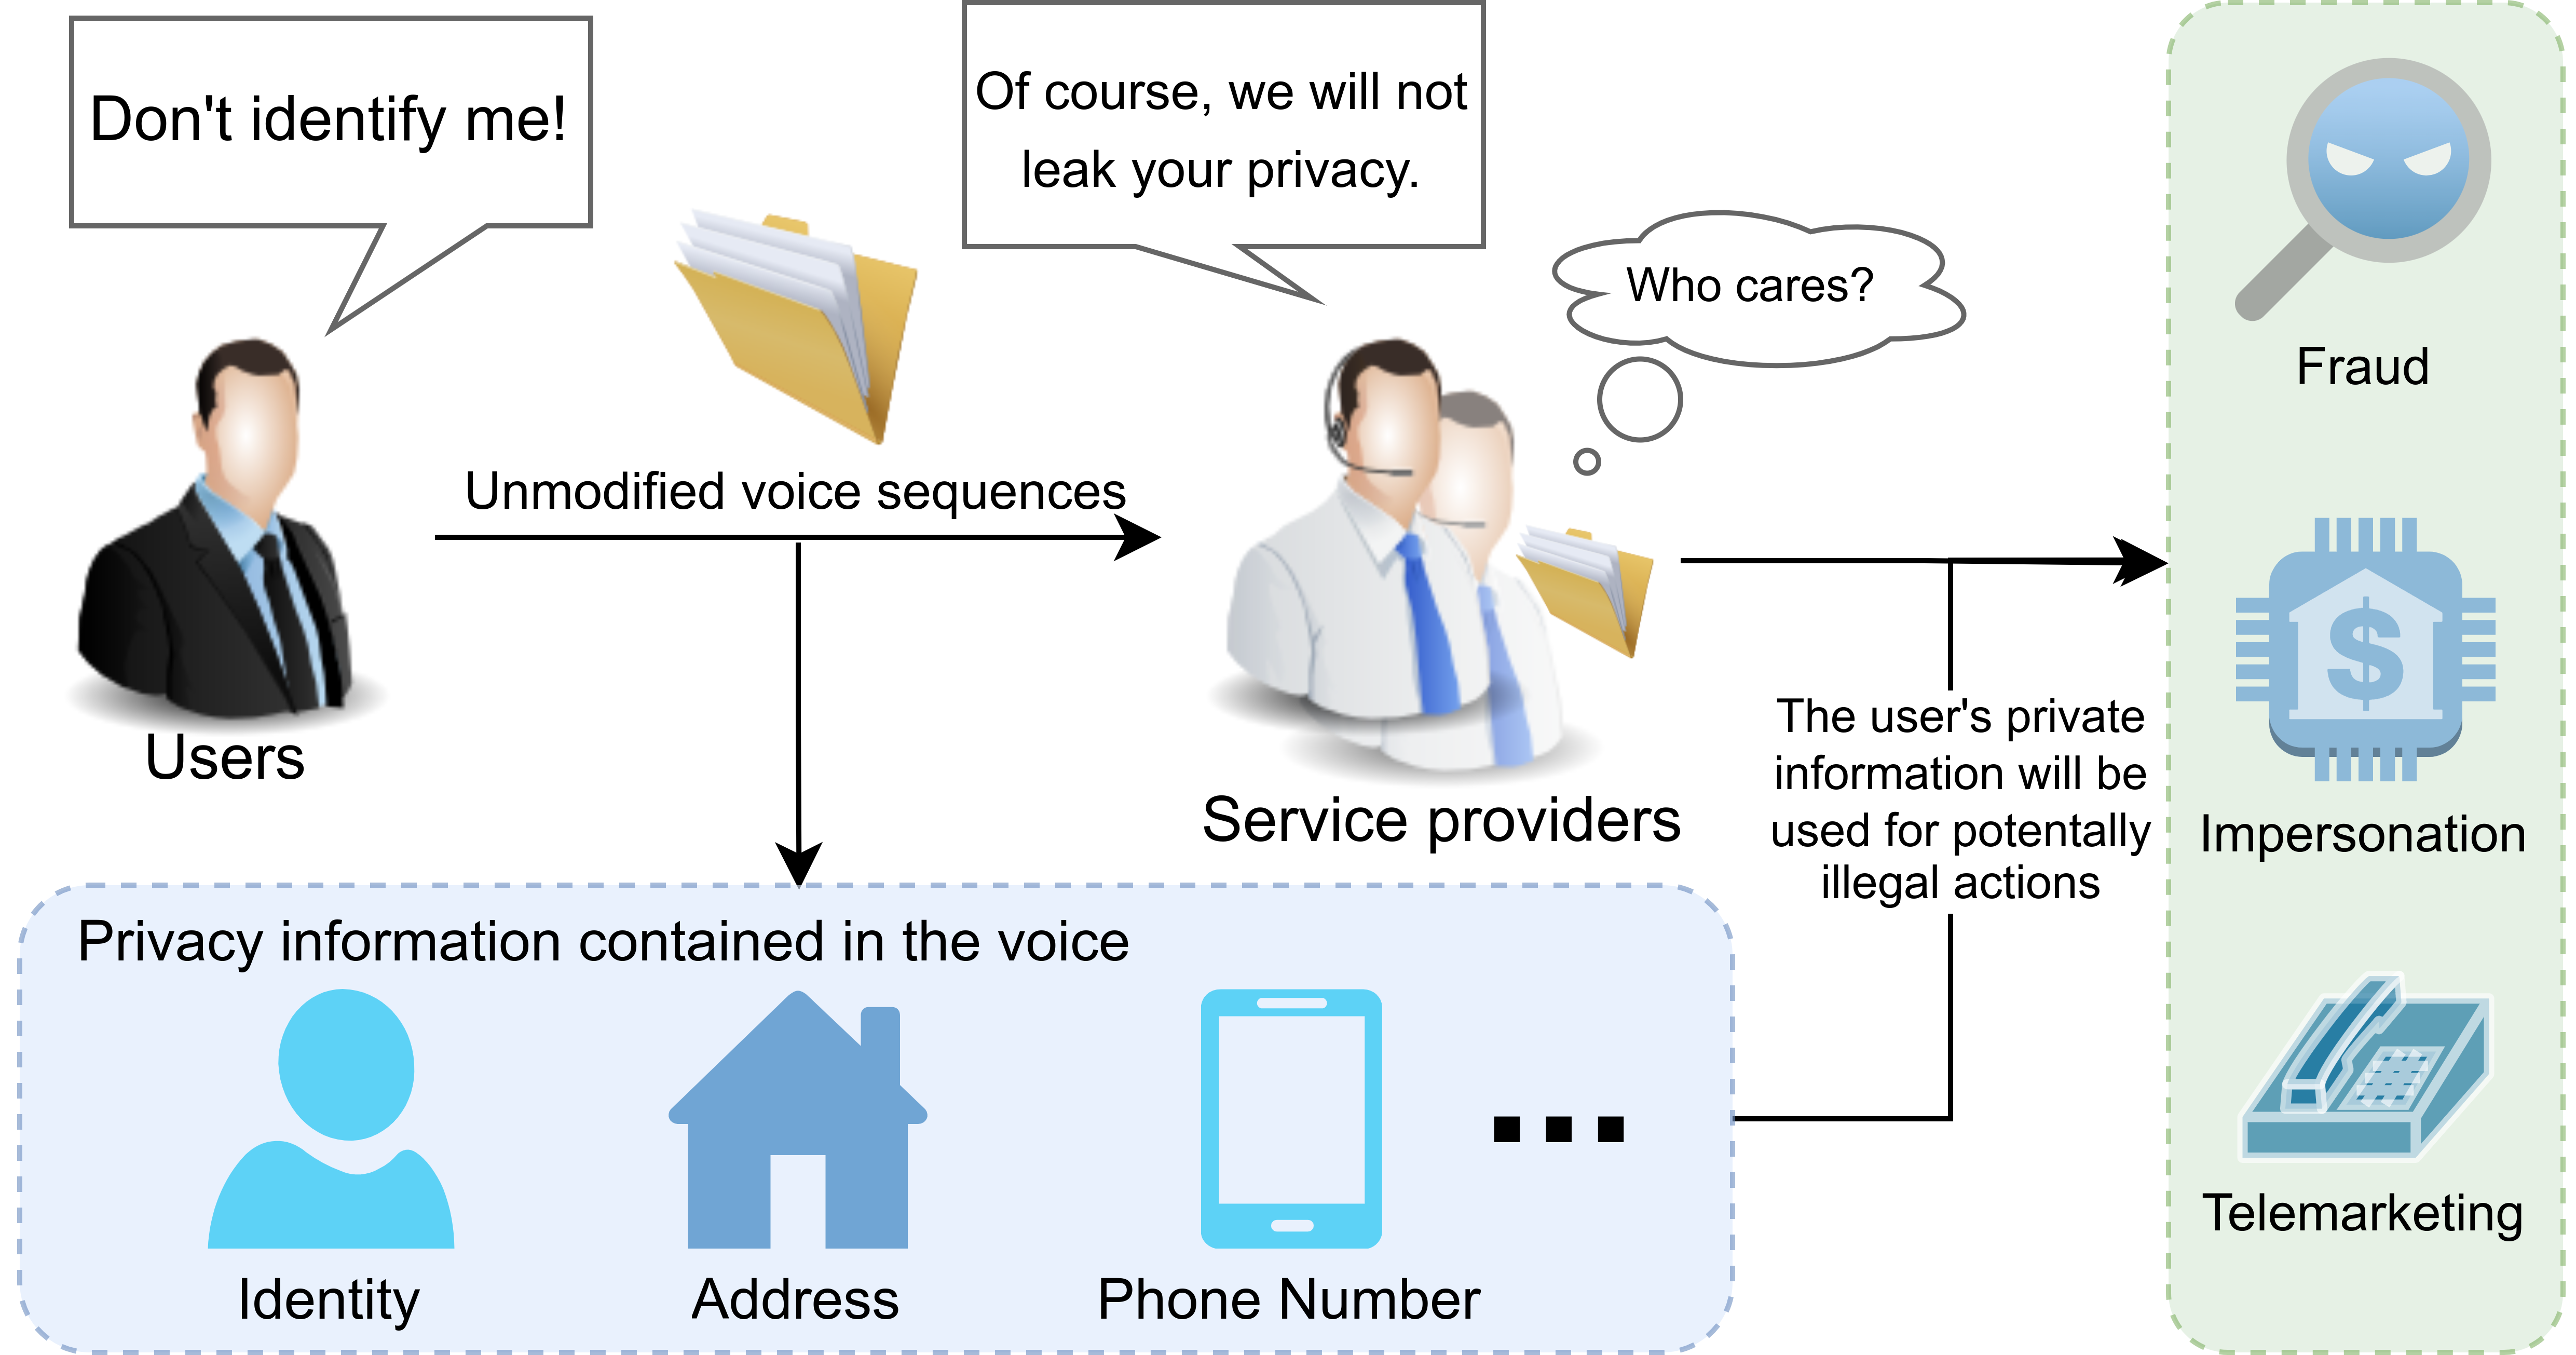
\includegraphics[width=8cm]{case2v3.png}}
    \caption{Is the speech service honest?}
    \label{case2}
\end{figure}

Ideally, an honest service provider would not use the raw recordings for anything other than the intended purpose. However, in reality this is not likely to be true for every single service provider. Such additional data, as mentioned before, may be used maliciously to identify the speaker and cause the exposure of user identity and other dangers as depicted in Fig. \ref{case2}. To alleviate such problem, many speech desensitization algorithms are being developed.

Conventional voice desensitization methods are believed to focus on two radically different areas: Content and Voiceprint. However, either areas show a certain degree of incompleteness and insufficient alleviation of potential adversaries.

Those focus on content desensitization employ methodologies to remove or replace voice segments that are detected to contain sensitive information. There are publicly available APIs\cite{a13} and dedicated softwares for this purpose\cite{a14}. As a safe method or the last resort, some may employ manual audio editing to achieve this goal, as there exists a number of softwares sufficient for this use case\cite{a15}.

However, such content removal algoritms are likely to involve certain pattern matching process on the textual content of these voice sequences, which is vulnerable to a number of cases where the actual sensitive content is obfuscated by environmental noises, not clearly spoken or even in different languages.

Other methods may apply distortion on entire voice sequences. Deep learning based methodologies are employed in both types of methods along with traditional algorithms\cite{a9, a10, a11}.

These methods are more robust in terms of mitigating voiceprint privacy concerns. However, they are likely to suffer from the potential failure to cleanly remove the relationship between the transformed and the original sequences. That is, there is still relevent information in the processed data that can be picked up by a well-designed recognition algorithm. Moreover, the sparsity of relevent information in voice signals opens up possibilities for a vast number of potential attacking methods.

It's notable that many approaches to bring privacy to remotely handled voice recordings combine these 2 ideas to provide better performance. There exists a number of active researches on this subject\cite{a8}. In this paper, we mainly focus on the vulnerabilities of voiceprint-handling desensitization models.

\begin{figure}[htbp]
    \centerline{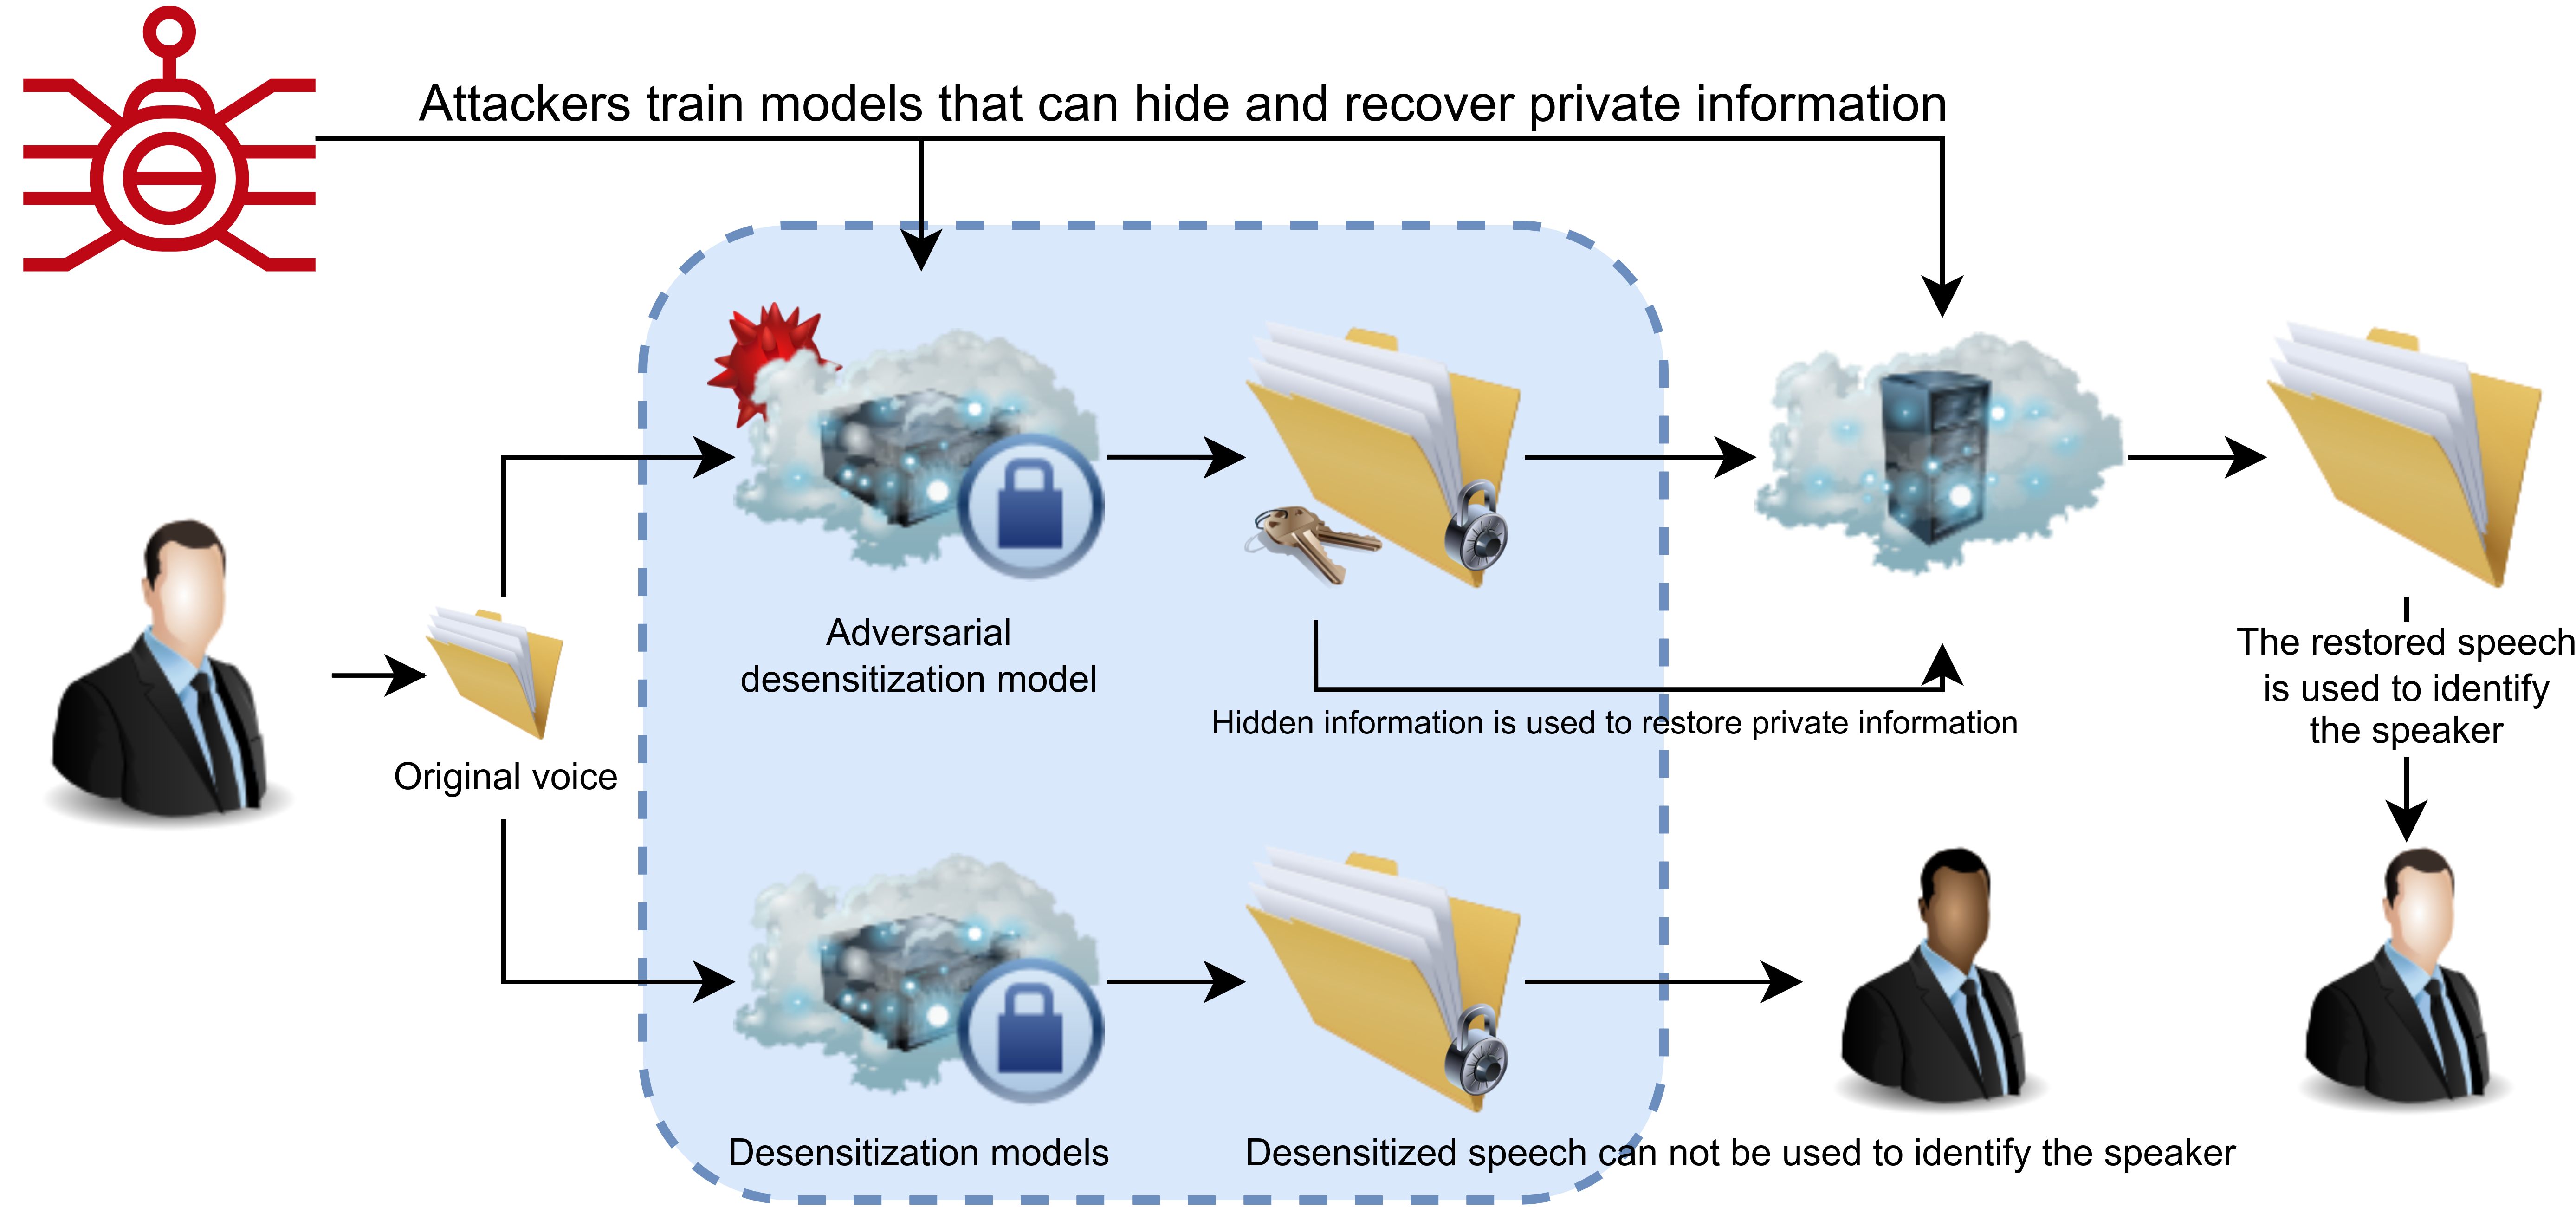
\includegraphics[width=8cm]{adversary.png}}
    \caption{Is the desensitization service honest?}
    \label{case4}
\end{figure}

It's unlikely to guarantee the absence of sensitive data in desensitized voices as just mentioned, which created its attack surface. Particularly, the desensitization method itself could also be modified to be able to embed additional information of original voice sequences in processed ones in different representations without excess degradation of performance\cite{a1}, as depicted in Fig. \ref{case4}. In this paper, we target this particular case and perform attack on a desensitization model.

In summary, this paper makes the following contributions.

\begin{itemize}

\item We demonstrate the adversarial case: Hiding sensitive data in desensitized voice sequences.

\item We present its concrete workflow: a novel, adversarial exploitation of voice desensitization frameworks that.

\item We conduct experiments on a particular voice transformation model with well-known voice samples. From them, we analyzed the performance and potential of this attack framework.

\end{itemize}
The rest of the paper consists related works, an detailed explanation of the proposed methodology, including the discussion of potential use cases and opportunities of future works.

\section{Related work}

\subsection{Adversary against desensitization}

There are researches on attacking privacy-preserving data transformation models. Some employ similar techniques that attempt to embed certain amount of data in sanitized data with modification to original deep-learning models and recover the original data after the exposure of sanitized data in public by victims. 

An notable instance among them works with images, targeting a privacy-preserving facial expression recognition algorithm, PPRL-VGAN. It sets up the attack with weak assumptions of user, who have white-box access to the attacked model. In order to achieve the adversary, its adversarial parts are embedded in the original model as additional layers or modification of existing layers, thus avoiding user's discovery.\cite{pprl-vgan,subvert}

However, there are much fewer works that propose adversaries against voice privacy preservation algorithms than facial image ones, even if the former is much more commonly adopted and deployed in production environment. The reason could involve the common misconception of voice-related technologies being mature or, even, complete.

\subsection{Voiceprint obfuscation}

Numerous research projects have been conducted for the preservation of voice privacy via the replacement of voiceprint. We consider these projects to fall in two categories: Traditional frequency-domain or voice tract analysis solutions and newer CNN-based voice transformation frameworks.

\subsubsection{Non deep learning based methods}

Those employ frequency-domain analysis use various preprocessing techniques to deduce certain features from the raw voice sequences. Then a statistical formula is applied to obfuscate these frequency features. Reversing the preprocessing steps previously applied, the transformed voice sequences is obtained.\cite{a9, a10, a11}

These methods are more likely to suffer from the issues mentioned before that they are not able to complete cut the connections to the original voice sequences or erasing the relevent features, thus they are not further discussed in this paper.

\subsubsection{Deep learning based methods}

There also exhibits a number of solutions utilizing neural networks. These methods are more likely to employ less sophisticated preprocessing means and focus on increasing the complexity of CNNs. These methods benefit from recent improvements made on NN-based content generation algorithms and transformer frameworks, such as the Diffusion models commonly used with graphics data.\cite{a8}

However, also as mentioned before, these models are at times likely to be vulnerable to adversaries that utilize the non-significant part of a voice sequence, namely stenography algorithms. Lacking dedicated mitigation of such issues, it's possible to retain the crucial private data in a different form without user's notice.

\section{Problem statement}

\subsection{Scenario}

In our scenario for this workflow, there exists two contradicting parties, users and the attacker.

\subsubsection{Users}

To users, the entire service is a black-box where they provide their raw voice sequences in exchange for services. Users can only verify the processed data that is actually sent to the remote servers.

\subsubsection{Attacker}

Attacker has access to a desensitization model to attack, either as a white-box with availability of source code or as a black-box with only public APIs. It want to modify this model or use another model as an add-in to embed features of original voice.

The only part where the attacker has access to raw sequences is the local program on user's device. Also, attacker has to ensure adequate difference between the raw sequences and the data sent to servers, which implies the recovery of original recordings is done remotely.

\subsubsection{Problem}

We consider the primary problem of our adversary generalizes to a specialized form of stenography where the desensitized sequence, as the carrier, carries the original counterpart the message. In this situation, the carrier and message share the same data type, format and textual content.

\subsection{Assumption}

As suggested before, the attacker has to use a form of stenography because it not only can not send the raw recordings over the network, but also may not have white-box access to the benign model to train or adjust for its purposes.

\subsection{Adversary model}

In order to complete such workflow, three distinct models are needed. They are explained in detail below, but they can also be summarized as following:

\begin{itemize}
    \item A \textbf{Benign model} to be attacked by. This model generates desensitized voice sequences that users would normally want to get from this black-box.
    \item A \textbf{Stenography model} to embed features of original voice sequences on the desensitized ones. The output sequences should trick users into believing it's clean desensitized ones.
    \item A \textbf{Extraction model} to extract the features that \textbf{Stenography model} hid in the voice sequences and recover original ones from them.
\end{itemize}

\section{Methodology}

\subsection{Benign model}

As suggested before, this model can either be in-house or outsourced. The source of benign model theoretically shows no significant difference in terms of the structure of adversary workflow we designed, but the performance differences may have an impact on the final results.

If the model is not outsourced, in which case the attacker can simply utilize the corresponding interfaces (HTTP APIs, for example), it need to train its own benign model. In order to demonstrate this particular case, we employ StarGAN-VC\cite{a3}, an non-parallel many-to-many voice conversion solution.

As a GAN-based model, StarGAN-VC's generator primarily optimizes for the following goal:

\begin{equation}
    \mathcal{L}_G
\end{equation}

\subsection{Stenography model}

The stenography model works as an add-on of the benign model to embed information of original voice into clean product of the benign model. It's notable that, users of this adversarial product are not intended to notice the presence of such stenography model that attempts to tamper the clean output.

Details are discussed in the following sections. However, the characteristics a stenography model needed to be adequate for this purpose can be summarized as follows:

\begin{itemize}
    \item \textbf{Integration with benign model}: The stenography model should not alienate the adversary workflow by requiring additional data, other than what is provided inside the black-box (the original voice sample and the desensitized one) or be able to be detected despite being inside the black-box.
    \item \textbf{Sufficient performance}: The stenography model should embed sufficient information for the extraction model to recover the original voice sequence, thus ensuring the possibility of the adversary. But it should also avoid excess modifications applied to the samples to reduce suspicion.
\end{itemize}

To prevent users from discovering the stenography logic, one can rely on the black-box nature of such type of desensitization services. However, users might have concern over potential security risks from a non-transparent process of desensitization.

An robust solution to this problem is to embed the stenography model into the benign one, as an additional set of layers for "post-processing", thus achieve the integration. In this way, the presence of stenography model could no longer be easily detected without dedicated research of behavior or even the source code and weights.

The benign desensitization model attempts to replace a certain amount of features of original voices with features that does not belong to the owner of them while the stenography model attempts to embed a certain amount of information of original features into the already-desensitized voices. It's very likely that during this process the overall audio quality will experience degradation to a certain degree. For this reason, the stenography model chosen for this purpose should be adequately powerful to avoid excessive modification to the voice output.

\subsection{Extraction model}

The extraction model accepts the final product from the combination of benign and stenography model, which is likely to be the voices user trusted to be desensitized, and attempts recovery of original voice from it.

\section{Experiment}

\subsection{Setup}

As mentioned before, we use StarGANVCDialectConversion, a StarGAN-VC implementation as the benign model to produce desensitized voices, Hide and Speak for stenography and extraction process. All our experiments are performed on a x86-64 based container-enabled Linux server with a NVIDIA Tesla V100 GPU. We used software packages required by each models, but with Python 1.10 and PyTorch 1.13, which are slightly newer.

 For convenience of further processes, we used voice samples from TM1, TM2, SF1 and SF2, speakers in the VCC2016 data set\cite{a16}, a well-known data set that is used by numerous projects and is versatile\cite{a17, a18}, as preferred by the configuration of benign model. The voices of TM1 is considered the original voices that contain sensitive information and ones of SF1, on the other hand, is considered desensitized. With this setup in mind, the experiment can be described as: Voices of TM1 are transformed into ones of SF1 by the benign model, and the stenography model takes the output and embed voice data of TM1, generating the final output. Extraction model then use the final output to recover the voices of TM1.

\subsection{Training}

We trained the models locally on the server. In order to streamline the experiment process while preserving the most accurate possible results, we avoid excess modifications to the models. Particularly, the benign model is trained to 200000 steps (~60 epochs), as the default settings. Similar approach is applied on the stenography model, that it is trained to preferred settings by the model authors.

\subsection{Generation}

It's necessary to clarify that, in order to achieve the maximum quantity of samples and prevent the quality of benign model from having excess impact on our overall process, we use the whole VCC2016 training set as the original voices. Each identity contains 162 samples, and we get 648 samples in total.

As a StarGAN-based model, our benign model is capable to transform a voice sequence from any known speakers to another. We consider the fact that the transformed voice belongs to other identity than the original speaker to be a form of desensitization, as mentioned before. Since each sample can be used to generate 3 sequences targeting different speakers, we get 1944 in total.

The remaining steps are straightforward. We used each sample generated by benign model to get a stenography one with the original sample associated with it. Finally we used the extraction model to recover each voices.

\subsection{Evaluation}

In order to generate creditable numbers for our voice samples that correctly reflect the amount of sensitive data, the identity of original speaker, we employed cloud-based voiceprint analysis solution provided by iFlyTek. After learning about the identity of four speakers in our domain, this service is able to generate 4 numbers for each voice sample, denoting the probability of the voice to belong to a particular speaker. iFlyTek suggests in the official manual that a score that is higher than 0.6 meant that the identity of a sample can be confirmed. We consider the identity with the highest score for a particular sample to be the classification made by this service.

\section{Results}

\subsection{Explanation}

Table I to IV presents the essential statistics of our results. All of the statistics are based on the score of each sample being classified into the original identity of their own. A higher score mean that our evaluation service, as mentioned before, deduces that the sample has a higher probability to belong to its original identity.

Each row contains statistics targeting the original identity of samples where their original identity is the speaker denoted in the header. Each column consists different types of results of statistical computation according to the following description:

\begin{itemize}
    \item \textbf{Mean} - Average value of scores. Higher values mean generally closer to the original speaker.
    \item \textbf{Certainty} - Ratio of scores being greater than 0.6, which means the sample can be confirmed to bear the same speaker as the original one. Higher values mean values are more definite.
    \item \textbf{Best} - Best value of scores.
    \item \textbf{Worst} - Worst value of scores. Closer value with \textbf{Best} means better stability.
    \item \textbf{Class Ratio (Abbrivated as "Class R.")} - Ratio of samples being classified into its original speaker, i.e. have the highest score being the original speaker, as mentioned before. Higher values mean higher probability an generic classification model will think the samples have the same identity of the original speakers.
\end{itemize}

\subsection{Analysis}

\begin{figure}[htbp]
    \centerline{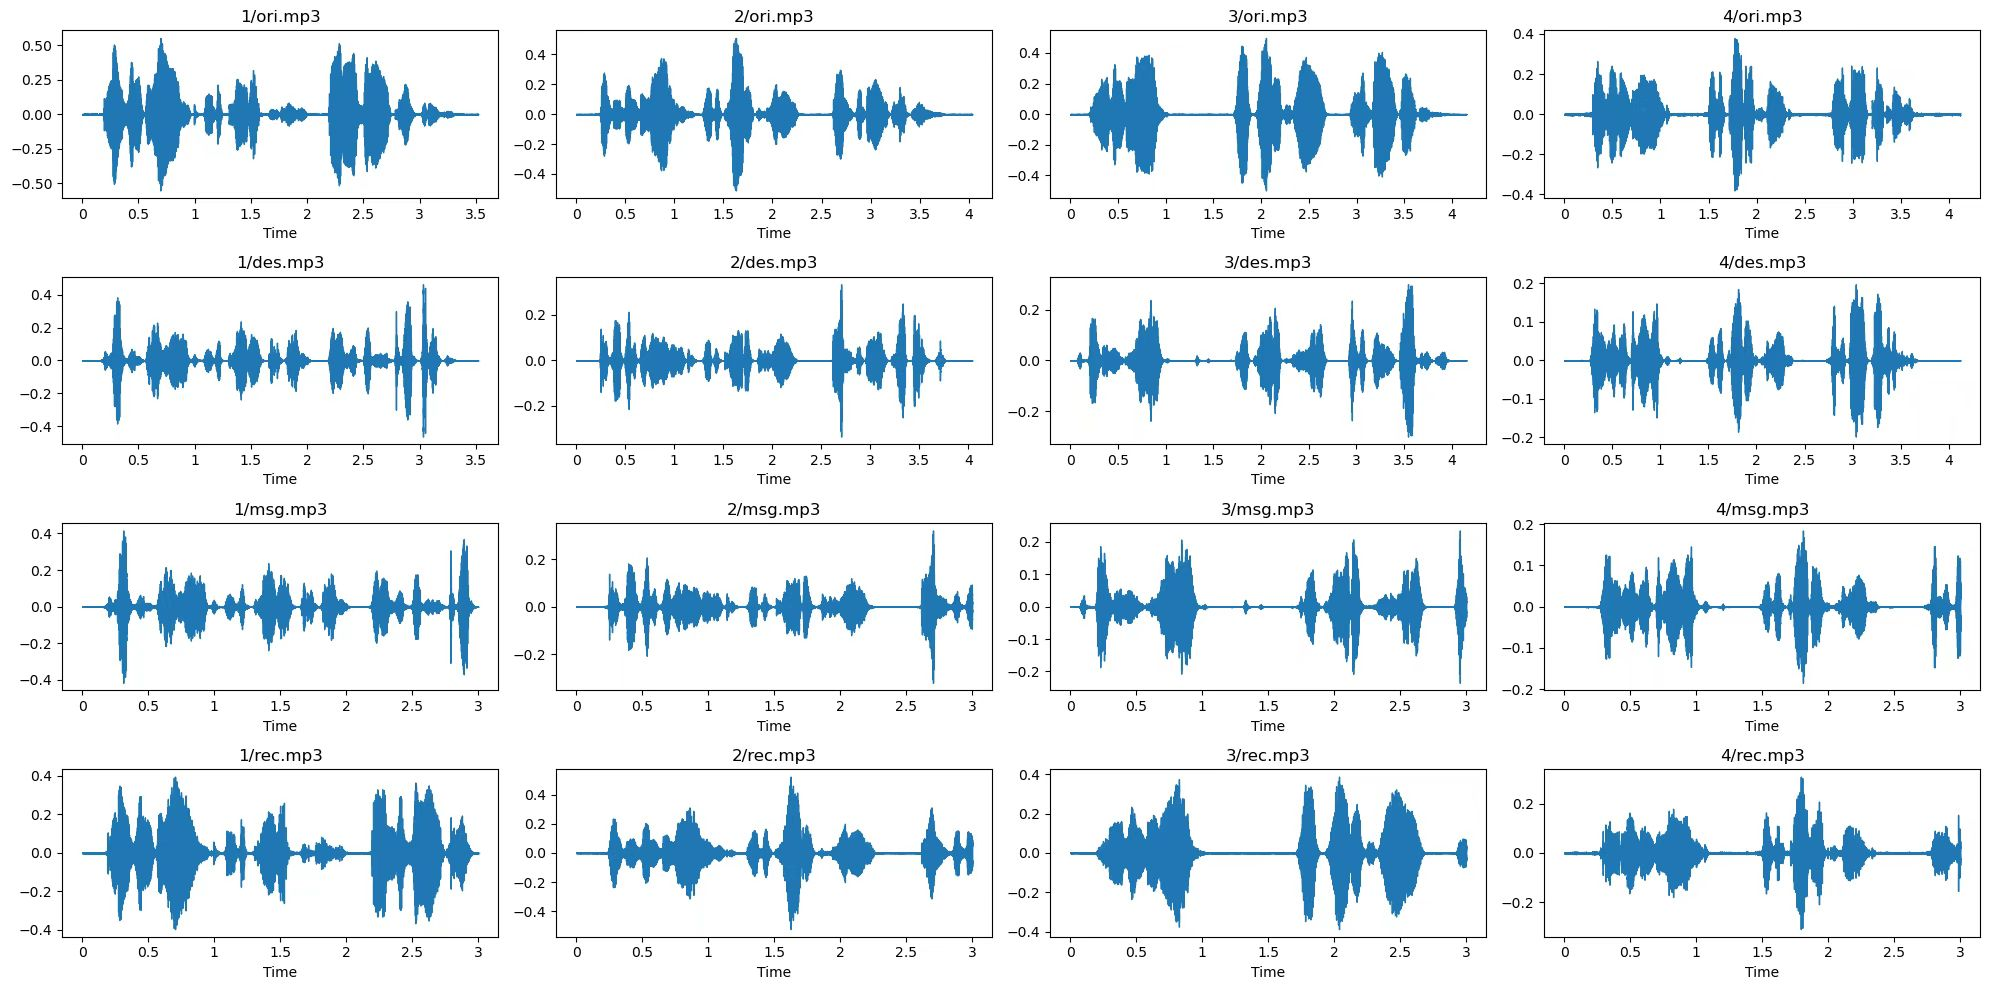
\includegraphics[width=8cm]{samp_wav.jpg}}
    \caption{4 sets of samples}
    \label{samp1}
\end{figure}

What is depicted in Fig. \ref{samp1} is 4 sets of voice samples in different stages of processing, original(\textbf{ori}), desensitized(\textbf{des}), stenography(\textbf{msg}) and extracted(\textbf{rec}). From which it's noticeable that the overall performance of this adversary is reasonable. Fig. \ref{chart_mean} displays the overall mean scores.
\subsubsection{Original samples}

According to Table I, all of the score statistics, except for the \textbf{Worst}, are close to 1, which is intended behavior for original samples. As the worst case, \textbf{Worst} is also close or greater than 0.6, which means that even this type of cases are confirmed to have the same identity as the original speaker. As a result, it's safe to confirm that both the benign model and the validation service are of desirable performance.

\subsubsection{Desensitized samples}

According to Table II, the overall score dropped drastically from over 0.8 to over 0.4. It can be argued that from the \textbf{Best} and \textbf{Class Ratio} numbers that there still exhibits a portion of samples that are classified into the original speaker. However, these type of classification results can not be trusted because they are vague, according to the close-to-zero \textbf{Certainty} value.

\subsubsection{Stenography samples}

Scores of stenography samples are similar to the desensitized ones, given the numerical changes of statistical numbers are mostly less than 0.1. However, the changes stenography model made to the samples did not cause any form of degradation of desensitization performance, but upgraded it instead.

Table V is the statistics of direct comparison between these two sets of samples. According to the \textbf{Minimum} value, it's still possible that the desensitization performance would suffer significant degradation from the stenography process, but from the \textbf{Mean} and \textbf{Variance} value we can see that the performance changes are even-spread.

It's highly likely that the changes are caused by the slight content degradation, i.e. perturbation, made by stenography model and would not strongly affect the overall performance of such adversary. We also performed manual audio quality tests on a random subset of this set of samples and confirmed that the degradation is not audible.

\subsubsection{Extracted samples}

As mentioned before, extracted samples are meant to be as close to the original samples as possible. As presented in Table IV, the values are slightly inferior than the original samples with the decrease of score within 0.1 to 0.2. However, despite the worsen results, the \textbf{Certainty} and \textbf{Class Ratio} are still well desirable, suggesting that the usability of these samples are comparable to the original ones, which declares the success of adversary.

\begin{table}[htbp]
    \centering
    \caption{Statistics of Original Samples}
    \begin{tabular}{|c|c|c|c|c|c|}
        \hline
        & \textbf{SF1} & \textbf{SF2} & \textbf{TM1} & \textbf{TM2} & \textbf{Mean} \\
        \hline
        \textbf{Mean} & 0.853889 & 0.837284 & 0.84537 & 0.837963 & 0.843627 \\
        \hline
        \textbf{Certainty} & 1.0 & 0.987654 & 1.0 & 1.0 & 0.996914 \\
        \hline
        \textbf{Best} & 0.95 & 0.94 & 0.94 & 0.94 & 0.9425\\
        \hline
        \textbf{Worst} & 0.6 & 0.56 & 0.6 & 0.61 & 0.5925\\
        \hline
        \textbf{Class R.} & 1.0 & 1.0 & 1.0 & 1.0 & 1.0\\
        \hline
    \end{tabular}
    \label{tab:st_org}
\end{table}

\begin{table}[htbp]
    \centering
    \caption{Statistics of Desensitized Samples}
    \begin{tabular}{|c|c|c|c|c|c|}
        \hline
        & \textbf{SF1} & \textbf{SF2} & \textbf{TM1} & \textbf{TM2} & \textbf{Mean} \\
        \hline
        \textbf{Mean} & 0.407654 & 0.440206 & 0.460556 & 0.417078 & 0.431374 \\
        \hline
        \textbf{Certainty} & 0 & 0.022634 & 0.047325 & 0.004115 & 0.18519 \\
        \hline
        \textbf{Best} & 0.58 & 0.64 & 0.62 & 0.62 & 0.62 \\
        \hline
        \textbf{Worst} & 0.22 & 0.23 & 0.27 & 0.21 & 0.24 \\
        \hline
        \textbf{Class R.} & 0.125514 & 0.236626 & 0.195473 & 0.012346 & 0.142490 \\
        \hline
    \end{tabular}
    \label{tab:st_des}
\end{table}

\begin{table}[htbp]
    \centering
    \caption{Statistics of Stenography Samples}
    \begin{tabular}{|c|c|c|c|c|c|}
        \hline
        & \textbf{SF1} & \textbf{SF2} & \textbf{TM1} & \textbf{TM2} & \textbf{Mean} \\
        \hline
        \textbf{Mean} & 0.387695 & 0.366070 & 0.412119 & 0.394115 & 0.390000 \\
        \hline
        \textbf{Certainty} & 0 & 0.002058 & 0 & 0 & 0.000515 \\
        \hline
        \textbf{Best} & 0.52 & 0.61 & 0.56 & 0.56 & 0.56 \\
        \hline
        \textbf{Worst} & 0.21 & 0.15 & 0.17 & 0.20 & 0.18 \\
        \hline
        \textbf{Class R.} & 0.119342 & 0.183128 & 0.189300 & 0.014403 & 0.126543 \\
        \hline
    \end{tabular}
    \label{tab:st_msg}
\end{table}

\begin{table}[htbp]
    \centering
    \caption{Statistics of Extracted Samples}
    \begin{tabular}{|c|c|c|c|c|c|}
        \hline
        & \textbf{SF1} & \textbf{SF2} & \textbf{TM1} & \textbf{TM2} & \textbf{Mean} \\
        \hline
        \textbf{Mean} & 0.681975 & 0.681728 & 0.695123 & 0.702593 & 0.690355 \\
        \hline
        \textbf{Certainty} & 0.901235 & 0.864198 & 0.950617 & 0.938272 & 0.913581 \\
        \hline
        \textbf{Best} & 0.81 & 0.81 & 0.81 & 0.85 & 0.82 \\
        \hline
        \textbf{Worst} & 0.44 & 0.47 & 0.53 & 0.46 & 0.48 \\
        \hline
        \textbf{Class R.} & 0.993827 & 1 & 1 & 0.993827 & 0.996914 \\
        \hline
    \end{tabular}
    \label{tab:st_rec}
\end{table}

\begin{figure}[htbp]
    \centerline{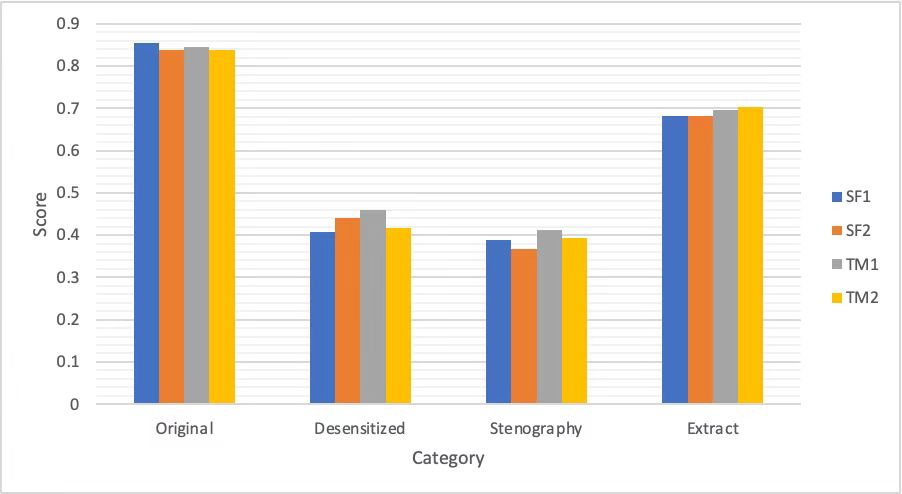
\includegraphics[width=8cm]{chart.jpg}}
    \caption{Chart Of Mean Scores}
    \label{chart_mean}
\end{figure}

\begin{table}[htbp]
    \centering
    \caption{Statistics of Differences Between Desensitized and Stenography Samples}
    \begin{tabular}{|c|c|}
        \hline
        \textbf{Mean} & 0.041373 \\
        \hline
        \textbf{Variance} & 0.010478 \\
        \hline
        \textbf{Maximum} & 0.37 \\
        \hline
        \textbf{Minimum} & -0.29 \\
        \hline
        \textbf{Maximum Absolute Value} & 0.37 \\
        \hline
        \textbf{Minimum Absolute Value} & 0 \\
        \hline
    \end{tabular}
\end{table}

\section{Discussion}

According to our experiments, it is safe to consider conventional acoustical-based or NN-based audio transforming solutions not sufficient for voice desensitization. Besides the StarGAN-VC solution we used, there exists many more such "voice changer" services on the Internet available for public use. One would consider these solutions secure because of the vast audible differences they made on its voice sequences. However, these solution exhibits potential of adversary with such method we demonstrated in this paper, which is not negligible. It's not likely that human ears can pick up subtle changes a stenography program made to certain parts of a voice sequence.

It's possible to avoid or mitigate risks of being attacked by such method. The most straightforward way to go is to avoid desensitization models from unknown or unsound sources. Due to the black-box nature of various proprietary services, it is not likely possible for users to have practical means to test these services for potential adversaries. When possible, users could train their own desensitization models. If the models are acquired from third-party, users should pay attention to the behaviour of model and the choice of training data set.

\section{Future Work}

In our experiment, we simply directed the voice sequence generated by the benign model to the stenography model. As mentioned before, this approach may not be sufficient in terms of stealthiness. Also, the overall storage consumption of this black box will increase significantly and the processing performance may not be ideal.

We believed that turning the stenography model into extra layers of benign model, eliminating the redundant audio encoding and decoding processes, can mitigate such problems while potentially increase the overall adversarial quality. In this way, the benign model can train in conjunction with the adversary model, taking advantage of intermediate representations of it. Moreover, this creates the potential of reducing the overall storage consumption and be less suspicious.

As another way to mitigate such problem, users can use various traditional or ML-based methods to apply inaudible perturbation on processed voices to attempt erasure of potential stenography while preserving high audio quality.

\section{Conclusion}

Targeting voice desensitization models based on generative NN models, we designed an adversary scheme that attempts to recover original voices from desensitized ones via stenography means, thus cause a privacy bleach. Our experiments prove this idea to be viable and the conventional solutions to be vulnerable to this type of adversary.

\end{CJK*}

\begin{thebibliography}{00}
    \bibitem{a1} N. Subramanian, O. Elharrouss, S. Al-Maadeed and A. Bouridane, "Image Steganography: A Review of the Recent Advances," in IEEE Access, vol. 9, pp. 23409-23423, 2021, doi: 10.1109/ACCESS.2021.3053998.
    \bibitem{a2} https://github.com/Didnelpsun/StarGanVCDialectConversion
    \bibitem{a3} Y. Li, X. Qiu, P. Cao, Y. Zhang, and B. Bao, “Non-parallel Voice Conversion Based on Perceptual Star Generative Adversarial Network,” Circuits Syst Signal Process, vol. 41, no. 8, pp. 4632–4648, Aug. 2022, doi: 10.1007/s00034-022-01998-5.
    \bibitem{a4} F. Kreuk, Y. Adi, B. Raj, R. Singh, and J. Keshet, “Hide and Speak: Towards Deep Neural Networks for Speech Steganography.” arXiv, Jul. 27, 2020. doi: 10.48550/arXiv.1902.03083.
    \bibitem{a5} N. Takahashi, M. K. Singh, and Y. Mitsufuji, “Source Mixing and Separation Robust Audio Steganography.” arXiv, Feb. 17, 2022. doi: 10.48550/arXiv.2110.05054.
    \bibitem{a6} Andreas Nautsch, Abelino Jiménez, Amos Treiber, Jascha Kolberg, Catherine Jasserand, Els Kindt, Héctor Delgado, Massimiliano Todisco, Mohamed Amine Hmani, Aymen Mtibaa, Mohammed Ahmed Abdelraheem, Alberto Abad, Francisco Teixeira, Driss Matrouf, Marta Gomez-Barrero, Dijana Petrovska-Delacrétaz, Gérard Chollet, Nicholas Evans, Thomas Schneider, Jean-François Bonastre, Bhiksha Raj, Isabel Trancoso, and Christoph Busch. 2019. Preserving privacy in speaker and speech characterisation. Comput. Speech Lang. 58, C (Nov 2019), 441–480. https://doi.org/10.1016/j.csl.2019.06.001
    \bibitem{a7} Kröger, J.L., Lutz, O.HM., Raschke, P. (2020). Privacy Implications of Voice and Speech Analysis – Information Disclosure by Inference. In: Friedewald, M., Önen, M., Lievens, E., Krenn, S., Fricker, S. (eds) Privacy and Identity Management. Data for Better Living: AI and Privacy. Privacy and Identity 2019. IFIP Advances in Information and Communication Technology(), vol 576. Springer, Cham.
    \bibitem{a8} Jaemin Lim, Kiyeon Kim, Hyunwoo Yu, and Suk-Bok Lee. 2022. Overo: Sharing Private Audio Recordings. In Proceedings of the 2022 ACM SIGSAC Conference on Computer and Communications Security (CCS '22). Association for Computing Machinery, New York, NY, USA, 1933–1946. https://doi.org/10.1145/3548606.3560572
    \bibitem{a9} J. Qian, H. Du, J. Hou, L. Chen, T. Jung and X. -Y. Li, "Speech Sanitizer: Speech Content Desensitization and Voice Anonymization," in IEEE Transactions on Dependable and Secure Computing, vol. 18, no. 6, pp. 2631-2642, 1 Nov.-Dec. 2021, doi: 10.1109/TDSC.2019.2960239.
    \bibitem{a10} Jianwei Qian, Haohua Du, Jiahui Hou, Linlin Chen, Taeho Jung, and Xiang-Yang Li. 2018. Hidebehind: Enjoy Voice Input with Voiceprint Unclonability and Anonymity. In Proceedings of the 16th ACM Conference on Embedded Networked Sensor Systems (SenSys '18). Association for Computing Machinery, New York, NY, USA, 82–94. https://doi.org/10.1145/3274783.3274855
    \bibitem{a11} J. Qian, F. Han, J. Hou, C. Zhang, Y. Wang and X. -Y. Li, "Towards Privacy-Preserving Speech Data Publishing," IEEE INFOCOM 2018 - IEEE Conference on Computer Communications, Honolulu, HI, USA, 2018, pp. 1079-1087, doi: 10.1109/INFOCOM.2018.8486250.
    \bibitem{a12} Nandwana, Mahesh Kumar, Julien van Hout, Mitchell McLaren, Allen R. Stauffer, Colleen Richey, Aaron D. Lawson and Martin Graciarena. “Robust Speaker Recognition from Distant Speech under Real Reverberant Environments Using Speaker Embeddings.” Interspeech (2018).
    \bibitem{a13} https://docs.aws.amazon.com/transcribe/latest/dg/pii-redaction.html
    \bibitem{a14} Vidizmo - Automatic audio redaction software. https://www.vidizmo/com/vidizmo-artificial-intelligence-solutions/redaction/
    \bibitem{a15} Audacity - Open source audio software. https://www.audacityteam.org/
    \bibitem{a16} T. Toda, L.-H. Chen, D. Saito, F. Villavicencio, M. Wester, Z. Wu, J. Yamagishi, "The Voice Conversion Challenge 2016," Proc. INTERSPEECH, pp. 1632-1636, 2016.
    \bibitem{a17} M. Wester, Z. Wu, J. Yamagishi, "Analysis of the Voice Conversion Challenge 2016 Evaluation Results," Proc. INTERSPEECH, pp. 1637-1641, 2016.
    \bibitem{a18} M. Wester, Z. Wu, J. Yamagishi, "Multidimensional scaling of systems in the Voice Conversion Challenge 2016," Proc. SSW9, pp. 40-45, 2016.
    \bibitem{a19} Siri - Voice assistant software. https://www.apple.com/siri/
    \bibitem{a20} Xiao Ai - Voice assistant software. https://xiaoai.mi.com/
    \bibitem{a21} iFly Input Method - Chinese/English input method software. https://srf.xunfei.cn
    \bibitem{a22} GBoard - Multilingual input method software. https://play.google.com/store/apps/details?id=com.google.android.inputmethod
    \bibitem{pprl-vgan} J. Chen, J. Konrad, and P. Ishwar, “VGAN-Based Image Representation Learning for Privacy-Preserving Facial Expression Recognition,” in 2018 IEEE/CVF Conference on Computer Vision and Pattern Recognition Workshops (CVPRW), Salt Lake City, UT, USA, Jun. 2018, pp. 1651–165109. doi: 10.1109/CVPRW.2018.00207.
    \bibitem{subvert} K. Liu, B. Tan, and S. Garg, “Subverting Privacy-Preserving GANs: Hiding Secrets in Sanitized Images,” AAAI, vol. 35, no. 17, pp. 14849–14856, May 2021, doi: 10.1609/aaai.v35i17.17743.
\end{thebibliography}

\end{document}
